\section{Architecture 101}

%\subsection{}

%\subsubsection{}

\textbf{Architectures:}
\begin{itemize}
	\item The art or practice of \textbf{designing} and \textbf{building} structure and especially habitable ones.
	\item A unifying or coherent \textbf{from} or \textbf{structure}
\end{itemize}

\textbf{Foundation for the study of Software Architecture / L. Wolf, 1992}

Software architecure principles can be \textbf{inherited} by appealing to several well-established architectural disciplines.

While the subject matter for the two is quite different, there are a number of intresting \textbf{architectural points} in building architecture that are suggestive for software architecture
\begin{itemize}
	\item multimple \textbf{views}
	\item architectural \textbf{styles}
	item style and \textbf{materials}
+\end{itemize}

\subsection{Multiple Views}

\subsubsection{Building Architecture}

\textbf{Building Architecture uses MULTIPLE VIEWS}

A building architect works with the customer by means of a number of different views in which sone \textbf{particular aspect of the building} is emphasized.

For exmaple, there are elevations and floor plans that give the \textbf{exterior views} and "\textbf{top-down}" views, respectively.

The elevation views may be supplemented by \textbf{contextual drawings} or even scale models to provide the customer with the look of the building in its context.

\subsubsection{Different Stakeholders}
Each perspective is not just a matter of different level or detail.

It is linked with \textbf{different natures} and \textbf{accountability}.

\begin{itemize}
	\item The \textbf{Owner} needs the building for a specific purpose. He/she does not know how, but hw/she knows perfectly \textbf{why}
	\item The \textbf{Architect} needs to project and formalize something that fit completely with owner's needs, to plan the \textbf{what}
	\item The \textbf{Builder} needs to design \textbf{how} the what will be built matching with natural laws and techological costraints
\end{itemize}

\subsubsection{\sout{Building} Software Architecture}

\textbf{\sout{Building} Software Architecture uses MULTIPLE VIEWS}

Different \textbf{type of users} will use Software Architecture: each of them will need a specific point of view.

A \textbf{Full Stack} developer needs to know how to write code inside the Architecture while a \textbf{Data Scientist} where are data they need.

\begin{center}
	\textit{Since the technology permits \textbf{destributing} large amounts of computing facilities in small packages to \textbf{remote location}, some kind of structure (or architecture) is imperative because \textbf{decentralization without structure is chaos}}.
\end{center}

\subsubsection{Zachman Framework for Building}

\begin{center}
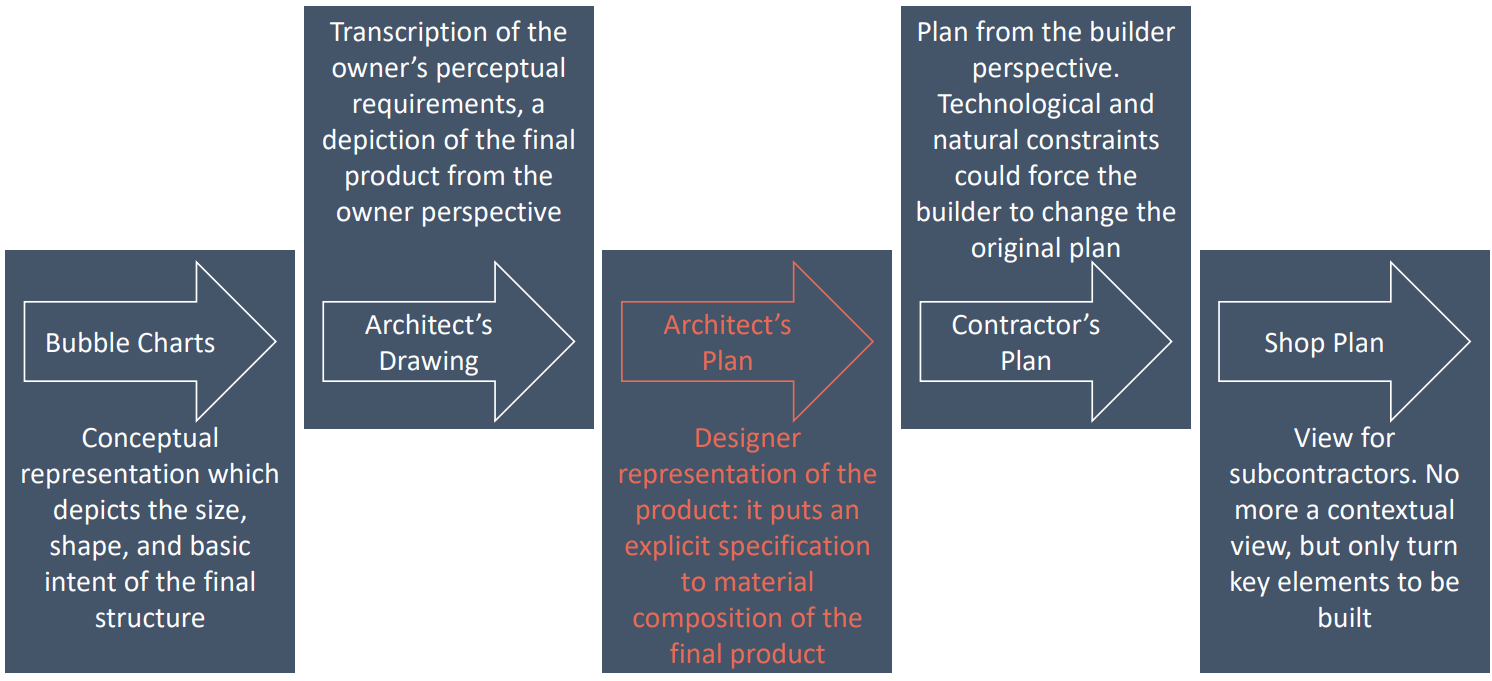
\includegraphics[scale=0.3]{1-zachman-framework-for-building}
\end{center}

\subsubsection{Zachman Framework for Information System}
\begin{center}
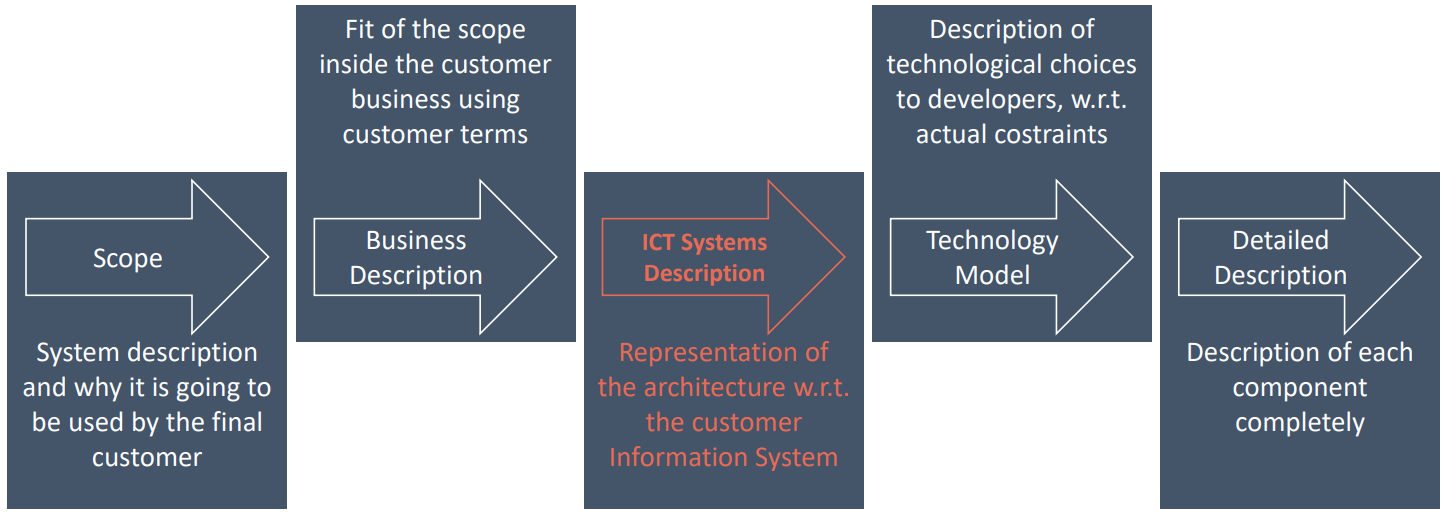
\includegraphics[scale=0.3]{2-zachman-framework-for-information-system}
\end{center}

\subsubsection{Different point of views}
Each perspective is not just a matter of different level of detail.

It is linked with \textbf{different natures} and \textbf{accountability}.

\begin{itemize}
	\item \textbf{Input-Process-Output}
	
	Product description in detail w.r.t. intended capabilities, appearance, and interactions with users
	
	\item \textbf{Entity-Relationship-Entity}
	
	<<Stuff things is made of>>, description of data in each building blocks
	
	\item \textbf{Node-Line-Node}
	
	Flows between each componenet
	
\end{itemize}













